\documentclass[border=3pt,tikz]{standalone}
\usetikzlibrary{positioning}
\begin{document}
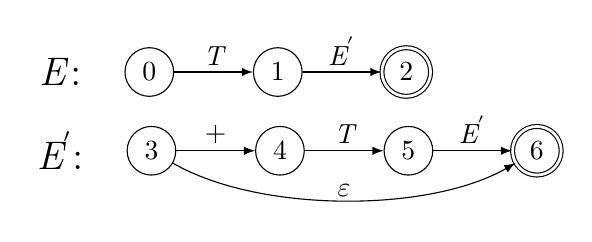
\begin{tikzpicture}
  % E
  \node (E) at (0,0) {\Large \textit{E}:};
  \node[circle,draw=black,right=1.21em of E] (zero) {0};
  \node[circle,draw=black,right=of zero] (one) {1};
  \node[circle,double,double distance=1pt,draw=black,right=of one] (two) {2};

  \path[-latex,draw]
  (zero) edge node[above=-1pt]{\(\textit{T}\)} (one)
  (one) edge node[above=-1pt]{\(\textit{E}^{'}\)} (two);

  % E'
  \node (ESkim) at (0,-1) {\Large \(\textit{E}^{'}\):};
  \node[circle,draw=black,right=1.21em of ESkim] (three) {3};
  \node[circle,draw=black,right=of three] (four) {4};
  \node[circle,draw=black,right=of four] (five) {5};
  \node[circle,double,double distance=1pt,draw=black,right=of five] (six) {6};

  \path[-latex,draw]
  (three) edge node[above=-1pt]{\(+\)} (four)
  (four) edge node[above=-1pt]{\(\textit{T}\)} (five)
  (five) edge node[above=-1pt]{\(\textit{E}^{'}\)} (six);

  \path[-latex,draw]
  (three) edge[out=330,in=210,max distance=3.6em] node[above=-2pt]{\(\varepsilon\)} (six);
\end{tikzpicture}
\end{document}
